\section{Technical Goals}
\label{sec:goals}
% DJS: For this initial paragraph, I would like us to try and answer the first few Heilmeyer questions, because these are critical components for DARPA. Let'ssee if we can succinctly address each question with an answer.
\thiswillnotshow{Heilmeyer Q1: What are you trying to do? Articulate your objectives using absolutely no jargon.}{
Imagine being able to simulate the group dynamics of a software engineering team with such fidelity that you could predict emergent programming misbehavior, catch bad code or wrong design choices before they become engrained into a project, and even identify social engineering.
Interpersonal interactions have an undeniable effect on software projects by influencing team behaviors and performance, and these social dynamics can frequently be difficult to isolate, measure, and assess.}
%exert unseen force on software projects that influence team behavior, reaction, and performance, and for those reasons getting them right is crucial to the success of a software development project.
\thiswillnotshow{Heilmeyer Q2: How is it done today, and what are the limits of current practice?}{
Currently, we determine the success of software development projects almost entirely on source code and their revision history, disregarding the complex group dynamics and social interactions that mold them.}
% Heilmeyer Q3: What is new in your approach and why do you think it will be successful?
\thiswillnotshow{Heilmeyer Q3: What is new in your approach and why do you think
it will be successful?}{We propose extending beyond the code, and utilizing the
rich social interactions that take place within projects' communication channels
(e.g., issue tracking, pull requests) to develop a set of generative
probabilistic models that predict emergent programming misbehavior.} These
models should be robust to changes in project activity as contributors,
time, circumstance, and interests frequently change in software development
projects.
% Heilmeyer Q4: Who cares? If you are successful, what difference will it make?
\thiswillnotshow{Heilmeyer Q4: Who cares? If you are successful, what difference will it make?}{The stakeholders of this project include individuals and organizations who rely on open source software to execute important strategic business and mission requirements, such as city governments, websites owners, and the Department of Defense (DOD). Stakeholders will be able to guard against compromised open source software before their integration into their critical systems.}

\subsection{Motivation}
\label{subsec:motivation}

The root of this project's motivation is the fact that the world is being
rebuilt in code. From the ever-growing Internet of Things (\textit{IoT}) to
advanced military operations, we are more dependent on critical software systems
than ever before.  Compounding on this alarming reality is the fact that
numerous critical systems integrate components from large open source projects
where it is difficult to monitor a type of behavior that is indicative of
adversaries rather than of the situation, such as the injection of
vulnerabilities and social engineering. Here, we will learn to capture
interesting group dynamics patterns, which are specific to active contributors
or specific to the projects in general, by introspecting large amounts of code
and social interaction histories in open-source \textit{IoT} platforms on
GitHub. Then, we will represent these patterns in a form that we can
algorithmically operationalize.

\subsection{Tasks}
\label{subsec:tasks}

The results of this project would lead to the development of social generative
models of software development that would allow for the prediction of emergent
programming misbehavior, and for the understanding of the internal group
dynamics that make projects fail or thrive. To accomplish this goal, we outline
the following discrete tasks;

\begin{itemize}
  \addtolength{\itemindent}{3.9mm}
  \item[Task 1:] Codifying emergent programming (mis)behavior. Identify common
  programming idioms that are specific to a group of developers or specific to a
  software development project, and annotating them with metadata using expert
  crowdsourcing.
  \item[Task 2:] Modeling social hierarchy, network structure, and relationships
  within existing communication channels. Extract member and group social
  hierarchy information based on project roles, interactions, and GitHub
  activity, and then infer network structure and relationships using theories of
  hierarchical network structure and centrality.
  \item[Task 3:] \unsure{\Huascar Task 4 covers this content.}{Social Engineering Detection. Analyze language components to
  extract features related to manipulation and persuasion in inter-personal
  interactions on communication channels.}
  \item[Task 4:] Social generative models of software development. Learn the
  natural features of a dataset (produced from previous tasks), whether
  categories or dimensions or something else entirely, using a generative
  adversarial network (GAN) approach.
  \item[Task 5:] Programming (mis)behavior linting. Leverage this GAN approach
  to predict programming (mis)behavior actions that could lead to defect-prone
  changes in open source projects. We can expect to eventually generate samples
  that depict entirely plausible programming (mis)behavior with security risks.
%   \item[Task 6:] Cognitive Model. Develop a model of cognitive burden and load
% % * <owen@soe.ucsc.edu> 2017-10-26T23:48:37.916Z:
% %
% % adding a programming language dimension to this model might be interesting, or at least instantiate it for multiple languages.  I would guess the cognitive burden would change depending what the compiler or runtime takes care of.  E.g., in Python, a programmer has to program defensively to ensure function arguments have the correct type, but the Java type checker handles this at compile time (unless casting).
% %
% % ^ <owen@soe.ucsc.edu> 2017-10-26T23:52:17.111Z.
%   based on code complexity, used programming language, team member interactions, and variables related to
%   cognition (such as individual circadian rhythms).
\end{itemize}

The interesting research question is how much we can generalize from open source
projects' data, on Github, to predict such risky behavior. One of our core
aspirations of this project is to develop algorithms and data-driven techniques
that endow computers with an understanding of programming behaviors in open
source projects but that are not too complex to perform efficient analysis. This
has implications for how programming (mis)behavior evidence we generate and use
to inform owners and users of open source projects.

\subsection{Predicting Programming (Mis)Behavior with GANs}
\label{subsec:fundamentals}

The ability to accurately predict programming (mis)behavior is critical for the
development of green linters. Traditional modeling methods use simple parametric
models and behavioral cloning. This project will adopt an imitation learning
method to learn from live observations from demonstrated (mis)behavior. This
method not only minimizes cascading errors intrinsic to previous modeling
methods, but also produces human-like behavior that is robust to activity
perturbations within open source projects.

Figure \ref{fig:outline} outlines our approach for producing data-driven
programming (mis)behavior linters. Our approach involves a four-stage pipeline.
First, we mine the revision history of a group of popular \textit{IoT} open
source projects, as well as these the social interactions among these projects'
contributors. Second, we learn from example demonstrations (without rewards)  a
discriminator and a generator for policies imitating human-like behavior. Third,
we put these artifacts together to use to produce a set of data-driven analyzers
that open source projects can install as plugins.  The last step involves
operationalizing these analyzers. This last step will result in the firing of
behavior linting events, which will inform project owners of emergent
programming misbehavior forming in their projects.

\begin{figure}[ht!]
\centering
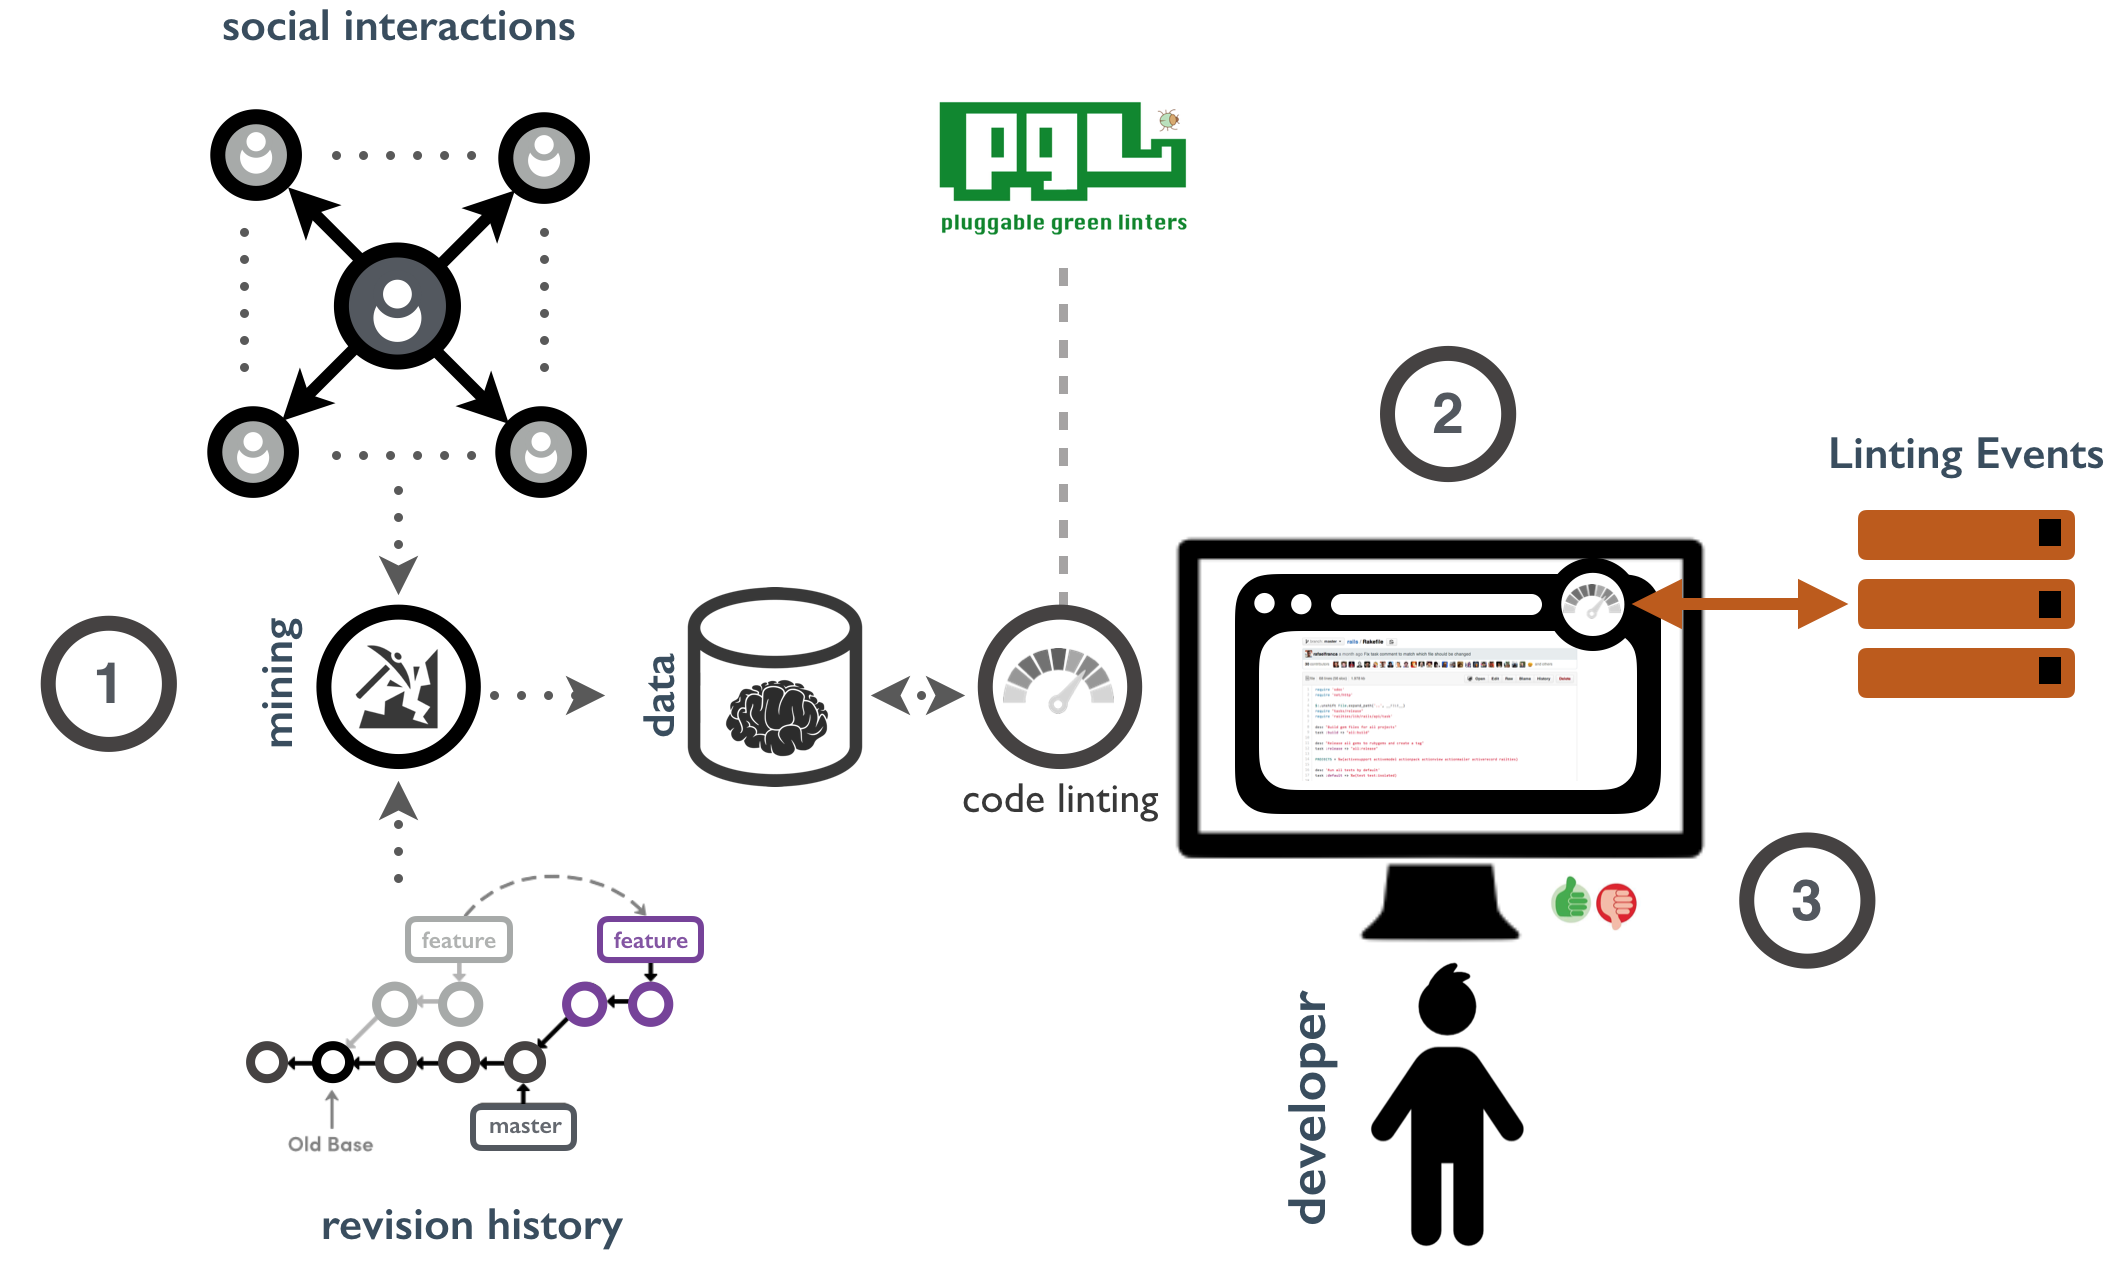
\includegraphics[width=11cm,height=4.5cm,keepaspectratio]
{images/greenlintersworkflow.png}
\caption{{\bfseries Project Outline and Strategy}.}
\label{fig:outline}
\end{figure}
